\section{ПРОЕКТИРОВАНИЕ СИСТЕМЫ}

\subsection{Архитектура системы}

Разрабатываемая система построена по многоуровневой клиент-серверной архитектуре с разделением на серверную и клиентскую части. Серверная часть реализована на языке Python с использованием фреймворка FastAPI и обеспечивает генерацию нагрузки, сбор метрик, управление подключениями к тестируемым СУБД, хранение истории тестов, а также управление профилями схем и логическими базами данных. Клиентская часть реализована на TypeScript с использованием фреймворка Next.js и предоставляет веб-интерфейс для управления тестированием, визуализации метрик в реальном времени и анализа результатов.

Взаимодействие между клиентской и серверной частями осуществляется по двум каналам. REST API используется для выполнения CRUD-операций с тестами, сценариями, подключениями, логическими базами данных и профилями схем, а также для запуска тестов и получения результатов. WebSocket обеспечивает двустороннюю связь для трансляции метрик производительности в реальном времени в ходе выполнения теста. Такая архитектура позволяет клиенту инициировать тестирование через HTTP-запрос и затем наблюдать за его ходом через WebSocket-соединение без необходимости периодического опроса сервера.

В процессе работы система взаимодействует с СУБД двух принципиально разных типов. Собственная СУБД системы~--- PostgreSQL~15, хранящая базу данных \texttt{project\_data},~--- предназначена для хранения истории тестов, конфигураций сценариев нагрузки, конфигураций подключений и результатов анализа. Вторая группа~--- целевые базы данных, работающие под управлением СУБД (PostgreSQL, MySQL, MariaDB), над которыми непосредственно проводятся нагрузочные тесты. Такое структурное разделение позволяет изолировать служебные данные от тестируемых сред и исключить искажение результатов из-за операций сохранения метрик в ходе прогона.

Архитектура системы включает девять основных компонентов. Центральным из них является модуль генерации нагрузки~--- ядро системы, реализующее параллельное выполнение SQL-запросов с заданным числом виртуальных пользователей, сбор метрик производительности и управление жизненным циклом теста. Модуль управления индексами отвечает за создание и удаление индексов базы данных до и после тестового прогона в соответствии со спецификацией конфигурации сценария нагрузки. Модуль управления подключениями предоставляет абстракцию подключения к различным СУБД, управление пулами соединений, формирование строк подключения и проверку доступности баз данных. Модуль управления состоянием БД обеспечивает сохранение состояния базы данных перед тестами с операциями записи, восстановление исходных данных после завершения теста и верификацию целостности восстановленного состояния.

Модуль генерации сценариев выполняет динамический анализ схемы подключённой базы данных и автоматически строит наборы параметризованных SQL-запросов для всех поддерживаемых типов нагрузки. Слой профилей и логических баз данных управляет шаблонами сценариев, профилями схем, конфигурациями сценариев нагрузки и логическими базами данных, объединяющими физические подключения под единой моделью данных. Модуль визуализации генерирует графики на основе временных рядов метрик и формирует сравнительные отчёты с применением статистических критериев. Модуль хранения содержит репозитории для работы с базой данных истории, реализующие операции создания, чтения, обновления и удаления записей о тестах, результатах, сценариях и профилях. Модуль сравнительного анализа представляет собой сервис для сопоставления результатов нескольких тестовых прогонов, вычисления описательной статистики и применения статистических критериев.

Каждый компонент реализован в виде отдельного модуля с чётко определённым интерфейсом взаимодействия, что обеспечивает возможность независимой модификации и тестирования компонентов. Архитектура системы допускает расширение перечня поддерживаемых СУБД путём добавления новых драйверов подключения без модификации остальной кодовой базы.

Взаимодействие компонентов системы представлено на рисунке~\ref{fig:architecture}. Клиентский браузер отправляет HTTP-запрос на запуск теста, сервер создаёт запись в базе данных истории и запускает фоновую задачу. Фоновая задача вызывает \texttt{LoadTester}, который через \texttt{DatabaseConnection} подключается к тестируемым СУБД, выполняет SQL-запросы и собирает метрики. Метрики передаются через callback-механизм в \texttt{WebSocket\-Manager}, который рассылает их через WebSocket всем подключённым клиентам и сохраняет в базе данных истории. Слой логических баз данных и профилей схем используется на этапе конфигурации: при выборе логической базы данных система автоматически разрешает привязанный профиль схемы и конфигурацию сценария нагрузки.

\begin{figure}
    \centering
    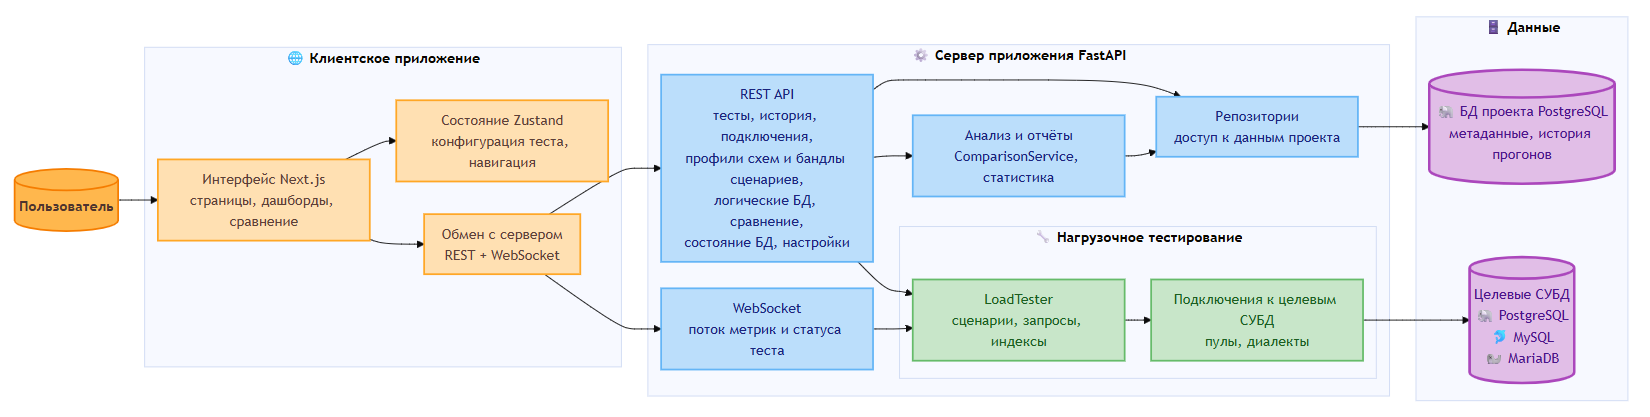
\includegraphics[width=0.9\linewidth]{img/arch.png}
    \caption{Взаимодействие компонентов системы}
    \label{fig:architecture}
\end{figure}

\subsection{Модуль генерации нагрузки и сбора метрик}

Модуль генерации нагрузки является центральным компонентом системы. При его проектировании определялись требования к параллельному выполнению SQL-запросов, точному замеру времени отклика, сбору системных и внутренних метрик СУБД, управлению индексами сценария, а также автоматическому управлению состоянием тестируемых баз данных.

Генерация нагрузки осуществляется с использованием асинхронной модели выполнения на базе библиотеки asyncio. Каждый виртуальный пользователь реализуется как асинхронная задача через \texttt{asyncio.Task}, выполняющая заданное число итераций SQL-запросов. Параллельное выполнение задач обеспечивается функцией \texttt{asyncio.gather()}, которая запускает все задачи одновременно и ожидает их завершения. Такой подход позволяет эффективно использовать ресурсы сервера без создания избыточного числа потоков операционной системы.

Для каждого выполняемого запроса фиксируется время отклика с использованием функции \texttt{time.perf\_counter()}, обеспечивающей высокую точность измерений. Результаты отдельных запросов накапливаются в структуре данных, из которой впоследствии вычисляются агрегированные метрики: среднее время отклика, процентили p50, p95, p99, минимальное и максимальное значения, а также количество ошибок.

Сбор метрик производительности организован в виде отдельного асинхронного цикла, выполняющегося параллельно с генерацией нагрузки. Цикл активируется с интервалом в одну секунду и на каждой итерации выполняет следующие действия:

\begin{enumerate}[label=\arabic*)]
    \item вычисляет агрегированные метрики за прошедший интервал времени на основе накопленных результатов запросов;
    \item собирает системные метрики через библиотеку psutil: загрузку центрального процессора, использование оперативной памяти, интенсивность дискового ввода-вывода, сетевой трафик;
    \item собирает внутренние метрики СУБД: коэффициент попаданий в кэш, количество ожиданий блокировок, количество взаимных блокировок, размеры таблиц;
    \item передаёт собранные метрики через callback-механизм для трансляции в реальном времени и сохранения в базе данных истории.
\end{enumerate}

Для трансляции метрик в реальном времени применяется callback-паттерн, обеспечивающий развязку между модулем генерации нагрузки и подсистемой передачи данных. Метрики сохраняются в базе данных истории в двух форматах: как точки временного ряда для построения графиков и как сырые выборки для последующего статистического анализа. Разделение форматов хранения позволяет применять к одним и тем же данным как визуализацию временны\'х рядов, так и непараметрические статистические критерии.

\subsubsection{Модуль управления индексами}

До начала основного этапа тестирования \texttt{IndexManager} создаёт индексы базы данных в соответствии со спецификацией выбранной конфигурации сценария нагрузки. Каждый индекс описывается объектом \texttt{ScenarioBundleIndex}, содержащим имя таблицы, перечень столбцов, тип индекса, признак уникальности и необязательное условие. После завершения тестового прогона \texttt{IndexManager} удаляет созданные индексы, восстанавливая исходное состояние схемы. Результат каждой операции фиксируется в объекте \texttt{IndexOperationResult}, содержащем информацию о времени создания и удаления каждого индекса, а также список ошибок.

\subsubsection{Алгоритм сохранения и восстановления состояния базы данных}

Тесты с операциями записи изменяют данные в тестируемой базе данных, что исключает повторяемость прогонов без предварительного сброса состояния. Для решения этой проблемы спроектирован модуль управления состоянием базы данных. Перед тестом анализируются SQL-запросы сценария: при наличии write-операций фиксируется снимок состояния базы данных, а после завершения теста данные восстанавливаются до исходного состояния. Для предотвращения конфликтов при параллельном тестировании нескольких баз данных одного типа предусмотрена блокировка на уровне типа СУБД, гарантирующая последовательное выполнение операций сохранения и восстановления.

В системе предусмотрены две взаимозаменяемые стратегии управления состоянием, выбор между которыми задаётся конфигурацией. Нативная стратегия использует штатные CLI-утилиты конкретной СУБД для создания дампа и его последующего восстановления --- этот подход обеспечивает максимальную точность и скорость операций. SQL-стратегия создаёт внутрибазовые копии таблиц средствами самой СУБД и не требует наличия внешних утилит, однако временно увеличивает объём данных в тестируемой базе. Если CLI-утилиты недоступны, система автоматически переключается с нативной стратегии на SQL-стратегию. После восстановления модуль верификации сравнивает число строк и контрольные суммы таблиц с зафиксированным до теста снимком и формирует отчёт о расхождениях при их обнаружении.

\subsubsection{Механизм параметризации запросов}

Для моделирования реалистичной нагрузки реализован механизм параметризации SQL-запросов. Каждый параметр запроса в конфигурации сценария нагрузки может быть сгенерирован одним из следующих способов:

\begin{enumerate}[label=\arabic*)]
    \item \texttt{random\_int} --- случайное целое число из заданного диапазона [min, max];
    \item \texttt{random\_from\_table} --- случайное значение из указанного столбца существующей таблицы базы данных;
    \item \texttt{sequential\_int} --- последовательное целое число, инкрементируемое на каждой итерации;
    \item \texttt{uuid} --- случайно сгенерированный UUID версии 4;
    \item \texttt{fixed} --- фиксированное значение, заданное в конфигурации параметра;
    \item \texttt{random\_string} --- случайная строка заданной длины из алфавитно-цифровых символов;
    \item \texttt{random\_date} --- случайная дата из заданного диапазона.
\end{enumerate}

Такой подход позволяет варьировать данные в запросах и избегать эффектов кэширования планов выполнения, которые могут искажать результаты тестирования. Значения типа \texttt{random\_from\_table} кэшируются на уровне ключа \texttt{db\_key:table:column} для снижения числа дополнительных запросов к БД в ходе теста.

Перед основным этапом тестирования выполняется фаза прогрева warmup, в ходе которой система выполняет серию предварительных запросов для инициализации кэшей и буферов СУБД. Это позволяет исключить влияние начальной инициализации на результаты основного этапа и получить более стабильные и воспроизводимые метрики производительности.

\subsection{Проектирование слоя сценариев и логических баз данных}

Для обеспечения гибкого сопоставления нагрузочных сценариев с конкретными базами данных в системе спроектирован трёхуровневый слой управления сценариями. Данная архитектура позволяет описать логику нагрузки независимо от конкретной СУБД и автоматически подбирать конкретные SQL-запросы при выборе подключения.

Нижний уровень образует шаблон сценария~--- логическое описание вида нагрузки без привязки к конкретной схеме данных. Шаблоны определяют семантику нагрузки: поддерживаются шесть встроенных типов~--- только чтение, только запись, смешанная лёгкая нагрузка, смешанная тяжёлая нагрузка, OLTP и OLAP. Встроенные шаблоны создаются автоматически при инициализации системы.

Средний уровень образует профиль схемы~--- описание структуры данных, общей для группы совместимых баз данных. Профиль связывает набор подключений с конкретной моделью данных и поддерживает три режима привязки: подтверждённый пользователем, ожидающий подтверждения и не определённый. При подключении новой базы данных система автоматически анализирует её схему и предлагает наиболее подходящий профиль с указанием степени уверенности определения.

Верхний уровень образует конфигурация сценария нагрузки~--- конкретная связка профиля схемы и шаблона сценария. Конфигурация содержит перечень параметризованных SQL-запросов и спецификацию индексов. Уникальность пары <<профиль + шаблон>> обеспечивается на уровне модели данных, что гарантирует отсутствие дублирующих активных конфигураций.

Конфигурации сценариев нагрузки формируются динамически на основе реальной схемы подключённой базы данных: система извлекает метаданные таблиц, столбцов и ключей и строит параметризованные SQL-шаблоны для каждого из шести типов нагрузки. При запуске теста конфигурация фиксируется в неизменяемом снимке, который сохраняется вместе с прогоном, обеспечивая воспроизводимость результатов.

Логическая база данных объединяет набор физических подключений под единой логической моделью данных и связывает их с конкретным профилем схемы. Это позволяет тестировать несколько экземпляров одной и той же схемы~--- например, PostgreSQL, MySQL и MariaDB с одинаковой структурой данных~--- в рамках одного прогона без дополнительной настройки сценариев. Система отслеживает совместимость схем подключённых баз данных и формирует отчёт о расхождениях при их обнаружении.

Спроектированный трёхуровневый слой обеспечивает масштабируемость системы: добавление новой схемы данных сводится к созданию профиля и генерации конфигураций сценариев нагрузки без изменения логики генерации нагрузки. Спроектированная архитектура формирует основу для перехода к следующему компоненту системы~--- подсистеме визуализации и сравнительного анализа.

\subsection{Подсистема визуализации и сравнительного анализа}

Подсистема визуализации предназначена для представления результатов нагрузочного тестирования в наглядном виде и обеспечения возможности сравнительного анализа нескольких тестовых прогонов.

Модуль сравнительного анализа поддерживает два режима работы. Режим per\_test предназначен для анализа одного тестового прогона с несколькими подключениями: выполняется попарное сравнение СУБД по метрикам задержки и пропускной способности с ранжированием подключений. Режим series ориентирован на анализ серии прогонов с различными уровнями нагрузки: строятся траектории изменения метрик по уровням и оцениваются характеристики масштабируемости.

В основе сравнительного анализа лежат непараметрические статистические критерии, применение которых обосновано характером распределения задержек: эмпирические распределения времени отклика, как правило, не являются нормальными и содержат выбросы. Тип критерия выбирается автоматически по результатам проверки нормальности выборки. При попарном сравнении нескольких СУБД применяется поправка на множественные сравнения для контроля уровня ложных открытий.

Аналитический отчёт формируется по структурированным правилам и включает краткое резюме с высокоуровневым вердиктом, анализ влияния параметров конфигурации на ключевые метрики, секцию практической значимости различий и конкретные рекомендации. Дополнительно автоматически выявляются характерные паттерны нестабильности производительности, деградации при масштабировании и высоких хвостовых задержек.

Для визуализации результатов сравнения предусмотрены три типа диаграмм: столбчатая диаграмма абсолютных значений задержки (среднее, p95, p99), диаграмма размаха для оценки разброса и асимметрии распределений, а также временно\'й график пропускной способности для выявления нестабильности и трендов. Детали программной реализации модуля сравнительного анализа рассмотрены в разделе~\ref{subsec:comparison_impl}.

\subsection{Модель данных}

Хранение данных системы организовано в базе данных PostgreSQL и включает следующие основные сущности.

TestRun --- запись о тестовом прогоне. Содержит уникальный идентификатор UUID, наименование, статус, конфигурацию теста в формате JSON (типы СУБД, число виртуальных пользователей, число итераций, время прогрева, идентификатор сценария), итоговую статистику в формате JSON, а также ссылку на логическую базу данных и поля управления состоянием базы данных: признак наличия операций записи, перечень затронутых таблиц, статус восстановления, длительность восстановления, ошибки восстановления, результат верификации. Связана с записями TestResult, TimeSeries и MetricSample через внешние ключи с каскадным удалением.

TestResult --- результаты тестирования для одной СУБД в рамках прогона. Содержит идентификатор тестового прогона, тип СУБД, идентификатор запроса, агрегированные метрики производительности в формате JSON (среднее время отклика, p50, p95, p99, TPS, количество ошибок, частота ошибок), системные метрики и внутренние метрики СУБД.

TimeSeries --- точки временного ряда для построения графиков. Каждая запись соответствует одному секундному интервалу тестирования и содержит: идентификатор тестового прогона, тип СУБД, временную метку, значения метрик (время отклика, TPS, загрузка CPU, использование RAM, дисковые IOPS, сетевой трафик, активные соединения, счётчик ошибок).

MetricSample --- сырые выборки метрик для статистического анализа. Каждая запись содержит: идентификатор тестового прогона, тип СУБД, ключ подключения, идентификатор запроса, тип выборки (request\_latency, throughput\_window), временную метку, задержку в миллисекундах, пропускную способность и признак ошибки.

DatabaseConnectionConfig --- конфигурация подключения к СУБД. Содержит тип СУБД, адрес сервера, порт, наименование базы данных, имя пользователя, зашифрованный пароль, группу подключений, идентификатор логической базы данных, идентификатор профиля схемы, а также результаты автоопределения профиля: имя определённого профиля, коэффициент уверенности и источник привязки.

SchemaProfile --- профиль схемы данных, описывающий структуру, общую для группы совместимых баз данных. Содержит наименование, описание, режим определения, ссылку на эталонное подключение, признак встроенного профиля. Связан с подключениями, логическими базами данных и конфигурациями сценариев нагрузки.

LogicalDatabase --- логическая база данных, объединяющая несколько физических подключений под единой моделью данных. Содержит наименование, описание, ссылку на профиль схемы, ссылку на эталонное подключение, статус привязки профиля, статус совместимости подключённых баз данных и отчёт совместимости. Связана с набором \texttt{DatabaseConnectionConfig} и с тестовыми прогонами через поле \texttt{logical\_database\_id} в \texttt{TestRun}.

ScenarioTemplate --- логический шаблон сценария нагрузки. Содержит строковый идентификатор, наименование, описание и признак встроенности. Связан с конфигурациями сценариев нагрузки через отношение <<один ко многим>>.

ScenarioBundle --- конкретная конфигурация сценария нагрузки, объединяющая профиль схемы и шаблон сценария. Содержит наименование, описание, источник генерации, признаки встроенности и активности. Уникальность активной пары <<профиль + шаблон>> обеспечивается частичным уникальным индексом. Связан с перечнями SQL-запросов и индексов.

ScenarioBundleQuery --- SQL-запрос внутри конфигурации сценария нагрузки. Содержит шаблон SQL-запроса, тип запроса, вес и порядковый номер выполнения. Связан с параметрами через отношение <<один ко многим>>.

ScenarioBundleParam --- параметр SQL-запроса внутри конфигурации сценария нагрузки. Содержит наименование параметра, тип генерации значений, диапазоны значений, ссылки на таблицу и столбец базы данных, текущее значение и шаг инкремента.

ScenarioBundleIndex --- спецификация индекса, связанного с конфигурацией сценария нагрузки. Содержит имя таблицы, перечень столбцов, тип индекса, наименование индекса, признак уникальности, условие (для частичных индексов) и описание. Используется \texttt{IndexManager} для создания и удаления индексов при выполнении тестового прогона.

Все основные сущности используют UUID в качестве первичных ключей для обеспечения глобальной уникальности идентификаторов и совместимости в распределённых сценариях. Высоконагруженные таблицы \texttt{TimeSeries} и \texttt{MetricSample} используют \texttt{BigInteger} для первичного ключа с автоинкрементом, что обеспечивает максимальную производительность вставки при потоковой записи метрик.

Модель данных представлена на ER-диаграмме на рисунке~\ref{fig:er_diagram}.

\begin{figure}
    \centering
    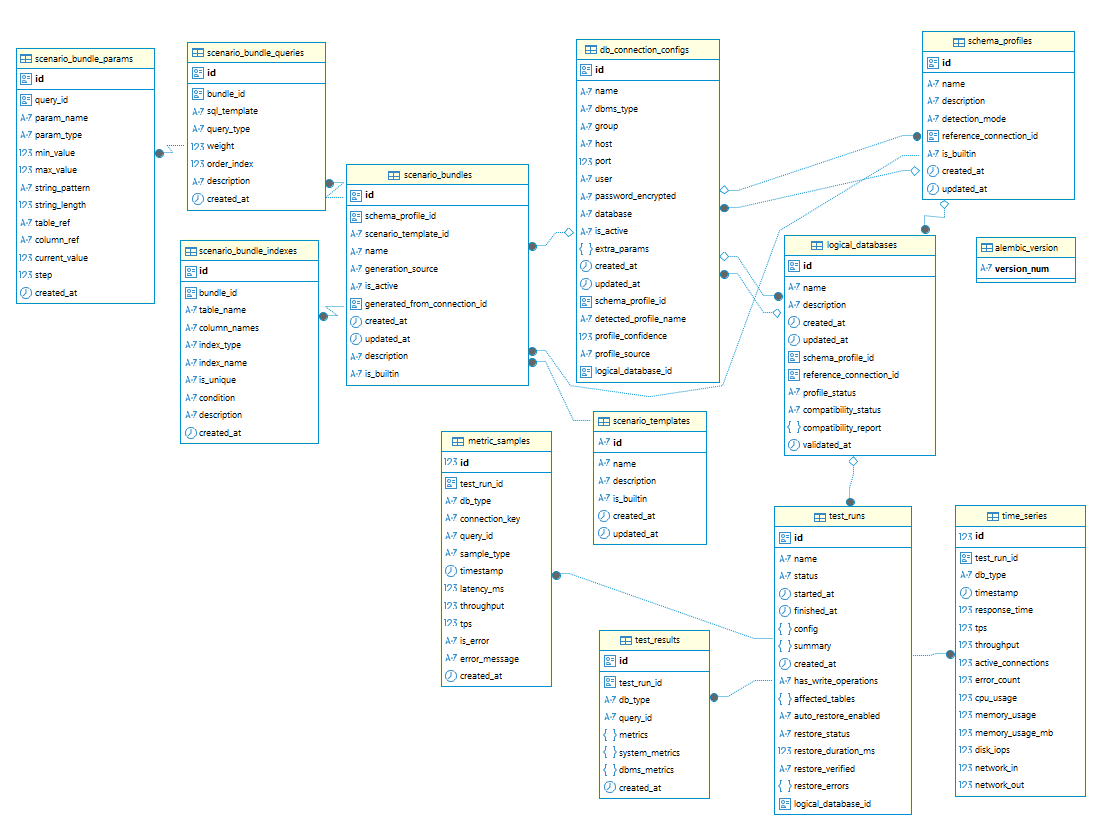
\includegraphics[width=0.9\linewidth]{img/er.png}
    \caption{ER-диаграмма модели данных системы}
    \label{fig:er_diagram}
\end{figure}

Проектирование модели данных с разделением на слой тестовых результатов и слой сценариев/профилей обеспечивает независимую развитие каждой части системы.

Спроектированная архитектура и модель данных создают необходимую основу для программной реализации системы, рассматриваемой в следующей главе.